\documentclass[12pt]{article}
\usepackage{fontspec}
\usepackage{xeCJK}
\setCJKmainfont[AutoFakeBold=2]{SimSun}
%\setCJKsansfont{SimHei}
\usepackage{amsmath, amssymb, amsthm}
\usepackage{geometry}
\usepackage{tikz}
\usepackage{fancyhdr}
%\setlength{\headheight}{15pt}
\usetikzlibrary{calc, intersections} % ABX 用於某些符號，若無可刪除
\usepackage{enumitem}
\usepackage{tkz-euclide}
\usepackage{subcaption}
\usepackage{float}
\counterwithin{figure}{section}
\counterwithin{figure}{subsection}
\usepackage[most]{tcolorbox}
\newtcolorbox{mybox}[4][證明]{
  empty,
  breakable,                % 支援跨頁
  sharp corners,
  left=#2+#3,               % 為左側標籤預留空間 (縮進)
  right=0pt, top=0pt, bottom=0pt,
  colback=white,
  % --- 加入以下這行來調整段距 ---
  before upper={\setlength{\parskip}{0.5em plus 0.2em minus 0.1em}},
  after={\vspace{#4}},
  % ---------------------------
  overlay unbroken and first={ % 在第一頁/未斷頁時繪製標籤
    \node[
      anchor=north west,
      draw, 
      inner sep=0pt,
      minimum width=#2,
      minimum height=1.6em, 
      font=\bfseries\boldmath
    ] at (frame.north west) {#1};
  }
}

\geometry{left=1.5cm, right=1.5cm, top=2cm, bottom=2cm}

% 設定頁首頁尾
\pagestyle{fancy}
\fancyhf{}
\renewcommand{\headrulewidth}{2pt}
\renewcommand{\thefigure}{\thesection-\arabic{figure}} % 主圖編號
\renewcommand{\thesubfigure}{圖 \thesubsection-\arabic{figure}} % 子圖變為 2-1
\captionsetup[figure]{labelformat=simple, labelsep=quad} 
\captionsetup[subfigure]{labelformat=simple, labelsep=quad} % 移除括號
\renewcommand{\figurename}{圖}
\lhead{廖汶鋒}
\chead{四點共圓}
\rhead{澳門培道中學}
\fancyfoot[C]{\thepage} % Centered footer
%\fancyfoot[L]{2026年2月7日} % Left footer

%\title{四點共圓}
%\author{廖汶鋒}
%\date{2026年2月7日}
\linespread{1.3}

% 定段落首行縮進（兩個中文字）
\setlength{\parindent}{2em}
\setlength{\headheight}{15pt} % 避免頁首高度警告
\begin{document}
\thispagestyle{fancy}  % 讓首頁也顯示頁首
%\maketitle
\begin{center}
    \textbf{\Large{四點共圓}}
\end{center}
四點共圓是競賽幾何題中的一個至關重要題種，是指不共線的四點位於同一圓上。
目前我們知道「任意不共線三點，有且只有一個通過此三點的圓」，但任意四點是否共圓則需要進一步判斷。
大部分讀者存在「幾何恐懼」的現象，就是因為沒有掌握好處理這類題目的方法。
本文將介紹多種常見的方法來處理四點共圓問題，並通過例題來說明這些方法的應用。

\section{與弦、弧、角相關的性質}
\begin{mybox}[垂徑定理]{6em}{1em}{0.5em}
    垂直於弦的直徑平分弦，並且平分弦所對的優弧及劣弧。
\end{mybox}
\begin{mybox}[圓周角定理]{7em}{1em}{0.5em}
    \begin{enumerate}[label= \arabic*., itemsep=0.2em]
        \item 同弧或等弧所對的圓周角是圓心角的一半；
        \item 同弦且分佈在弦的同側的圓周角相等；
        \item 同弦且分佈在弦的異側的圓周角互補。
    \end{enumerate}
\end{mybox}
\begin{mybox}[圓冪定理]{6em}{1em}{0.5em}
    圓$\Gamma$上存在四個不同點$A$、$B$、$C$、$D$，設直線$AB$與直線$CD$交於點$P$，
    則有$\overrightarrow{PA}\cdot\overrightarrow{PB}=\overrightarrow{PC}\cdot\overrightarrow{PD}$。
    \begin{enumerate}[label= \arabic*., itemsep=0.2em]
        \item 相交弦定理；
        \item 兩割線定理；
        \item 切割線定理。
    \end{enumerate}
\end{mybox}
\begin{mybox}[弦切角定理]{7em}{1em}{0.5em}
    圓$\Gamma$上存在兩個不同點$A$、$B$，設直線$PB$與圓$\Gamma$相切，那麼任取圓$\Gamma$上且不在$\angle{PBA}$內部的一點$C$，都有$\angle{PBA}=\angle{BCA}$。
\end{mybox}
\newpage
\section{四點共圓常用判定方法}
\subsection{圓的定義}
\begin{mybox}[定理]{4em}{1em}{1em}
    $A$、$B$、$C$、$D$四點共圓的充分必要條件是存在一點$O$使得$OA=OB=OC=OD$。
\end{mybox}
\subsection{圓周角}
\begin{mybox}[定理]{4em}{1em}{0.5em}
    對於不共線的四點$A$、$B$、$C$、$D$
    \begin{enumerate}[label= (\roman*.), itemsep=0.3em]
        \item 若$B$、$D$同時位於直線$AC$的同側，則$A$、$B$、$C$、$D$四點共圓的充分必要條件是$\angle{ABC}=\angle{ADC}$；
        \item 若$B$、$D$分別位於直線$AC$的異側，則$A$、$B$、$C$、$D$四點共圓的充分必要條件是$\angle{ABC}+\angle{ADC}=180^{\circ}$。
    \end{enumerate}
    \begin{figure}[H]
        \centering
        \begin{subfigure}[b]{0.45\textwidth}
            \centering
            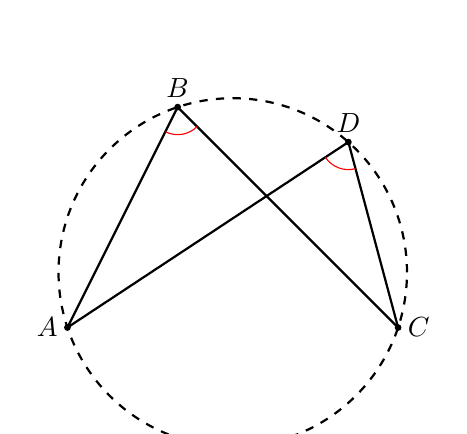
\begin{tikzpicture}[scale=0.7]
                \tkzDefPoint(0,4){B}
                \tkzDefPoint(-2,0){A}
                \tkzDefPoint(4,0){C}
                \tkzCircumCenter(A,B,C) \tkzGetPoint{O}
                \tkzDefPointBy[rotation=center O angle -60](B) \tkzGetPoint{D}
                \tkzDrawCircle[black, thick, dashed](O,B)
                \tkzDrawPoints[fill=black](A,B,C,D)
                \tkzDrawSegments[black, thick](A,B B,C A,D D,C)
                \tkzLabelPoints[above](B,D)
                \tkzLabelPoints[left](A)
                \tkzLabelPoints[right](C)
                \tkzMarkAngle[color=red, size=0.5](A,B,C)
                \tkzMarkAngle[color=red, size=0.5](A,D,C)
            \end{tikzpicture}
            \caption{$B$、$D$同時位於直線$AC$的同側}
            \label{fig:Angle_s2.2-1}
        \end{subfigure}
        \stepcounter{figure}
        \hfill % 在兩圖之間加入彈性間距
        \begin{subfigure}[b]{0.45\textwidth}
            \centering
            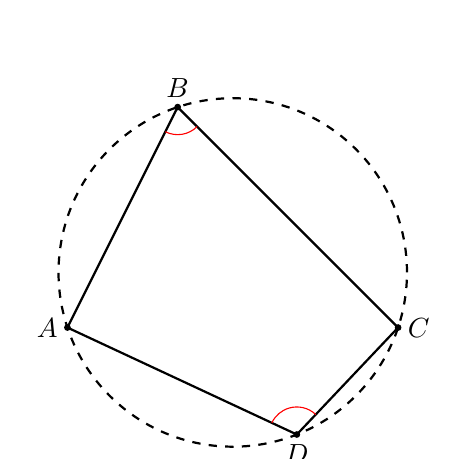
\begin{tikzpicture}[scale=0.7]
                \tkzDefPoint(0,4){B}
                \tkzDefPoint(-2,0){A}
                \tkzDefPoint(4,0){C}
                \tkzCircumCenter(A,B,C) \tkzGetPoint{O}
                \tkzDefPointBy[rotation=center O angle -50](C) \tkzGetPoint{D}
                \tkzDrawCircle[black, thick, dashed](O,B)
                \tkzDrawPoints[fill=black](A,B,C,D)
                \tkzDrawSegments[black, thick](A,B B,C A,D D,C)
                \tkzLabelPoints[left](A)
                \tkzLabelPoints[above](B)
                \tkzLabelPoints[right](C)
                \tkzLabelPoints[below](D)
                \tkzMarkAngle[color=red, size=0.5](A,B,C)
                \tkzMarkAngle[color=red, size=0.5](C,D,A)
            \end{tikzpicture}
            \caption{$B$、$D$分別位於直線$AC$的異側}
            \label{fig:Angle_s2.2-2}
        \end{subfigure}
    \end{figure}
\end{mybox}
\begin{mybox}[證明]{4em}{1em}{0.5em}
    因為定理的必要性可由圓內接四邊形的性質得出，所以只需證明定理的充分性就可。
    \begin{enumerate}[label= (\roman*.), itemsep=0.3em]
        \item 設射線$AD$交$\triangle{ABC}$外接圓於點$D'\neq A$，由圓內接四邊形的性質可知
        $$
            \angle{AD'C}=\angle{ABC}
        $$
        結合已知條件$\angle{ADC}=\angle{ABC}$，得出$\angle{AD'C}=\angle{ADC}$。

        利用三角形外角和不相鄰的內角的關係可得
        $$
            \angle{D'CD}=\left|\angle{ADC}-\angle{AD'C}\right|=0
        $$
        由此可得$D'=D$，即$A$、$B$、$C$、$D$四點共圓。
        \item 設射線$AD$交$\triangle{ABC}$外接圓於點$D'\neq A$，由圓內接四邊形的性質可知
        $$
            \angle{ABC}+\angle{AD'C}=180^{\circ}
        $$
        結合已知條件$\angle{ABC}+\angle{ADC}=180^{\circ}$，得出$\angle{AD'C}=\angle{ADC}$。

        利用三角形外角和不相鄰的內角的關係可得
        $$
            \angle{D'CD}=\left|\angle{ADC}-\angle{AD'C}\right|=0
        $$
        由此可得$D'=D$，即$A$、$B$、$C$、$D$四點共圓。
    \end{enumerate}
\end{mybox}
\begin{mybox}[定理簡化]{6em}{1em}{0.5em}
    把以上定理用有向角去重新改寫
    \begin{enumerate}[label= (\roman*.), itemsep=0.3em]
        \item 若$B$、$D$同時位於直線$AC$的同側，則$A$、$B$、$C$、$D$四點共圓的充分必要條件是$\measuredangle{ABC}=\measuredangle{ADC}$；
        \item 若$B$、$D$分別位於直線$AC$的異側，則$A$、$B$、$C$、$D$四點共圓的充分必要條件是$\measuredangle{ABC}+\measuredangle{CDA}=180^{\circ}$。
    \end{enumerate}
    注意(ii.)中有$\measuredangle{CDA}=-\measuredangle{ADC}$，所以(ii.)可以改寫成$\measuredangle{ABC}=180^{\circ}+\measuredangle{ADC}$。

    再結合有向角的周期性（$\measuredangle{A}$和$\measuredangle{A}+180^{\circ}k,\ k\in\mathbb{Z}$為同一角），圓周角的判定定理可以歸納成以下一條法則：
    \begin{quotation}
        $A$、$B$、$C$、$D$四點共圓當且僅當$\measuredangle{ABC}=\measuredangle{ADC}$
    \end{quotation}
\end{mybox}
\begin{mybox}[例題\thesubsection-1]{6em}{1em}{0.5em}
    在$\triangle{ABC}$中，$D$和$E$分別是$AB$和$AC$上的點，滿足$CD\perp AB$和$BE\perp AC$。記$CD$與$BE$的交點為$H$，求證：
    \begin{enumerate}[label = (\roman*.), itemsep=0.3em]
        \item $B$、$C$、$D$、$E$四點共圓；
        \item $A$、$D$、$E$、$H$四點共圓。
    \end{enumerate}
\end{mybox}
\begin{mybox}[解]{3em}{1em}{0.5em}
    \begin{figure}[H]
        \begin{subfigure}[b]{\textwidth}
            \centering
            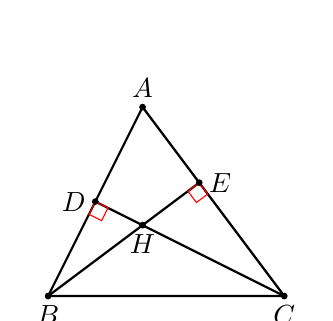
\begin{tikzpicture}[scale=0.6]
                \tkzDefPoints{0/4/A, -2/0/B, 3/0/C}
                \tkzDefPointBy[projection=onto A--B](C) \tkzGetPoint{D}
                \tkzDefPointBy[projection=onto A--C](B) \tkzGetPoint{E}
                \tkzDrawPolygon[black, thick](A,B,C)
                \tkzDrawSegments[black, thick](C,D B,E)
                \tkzMarkRightAngle[color=red, size=0.3](B,D,C)
                \tkzMarkRightAngle[color=red, size=0.3](B,E,C)
                \tkzInterLL(B,E)(C,D) \tkzGetPoint{H}
                \tkzDrawPoints[fill=black](A,B,C,D,E,H)
                \tkzLabelPoints[above](A)
                \tkzLabelPoints[below](B,C,H)
                \tkzLabelPoints[left](D)
                \tkzLabelPoints[right](E)
            \end{tikzpicture}
            \label{fig:Angle_s2.2-3}
            \caption{例題2.2-1示意圖}
        \end{subfigure}              
    \end{figure}
    \begin{enumerate}[label= (\roman*.), itemsep=0.3em]
        \item 本題可以用圓的定義或圓周角來解
        \begin{enumerate}[label = 方法 \arabic*：]
            \item 圓的定義
            \begin{figure}[H]
                \begin{subfigure}[b]{\textwidth}
                    \centering
                    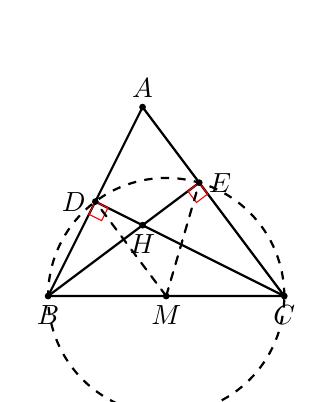
\begin{tikzpicture}[scale=0.6]
                        \tkzDefPoints{0/4/A, -2/0/B, 3/0/C}
                        \tkzDefPointBy[projection=onto A--B](C) \tkzGetPoint{D}
                        \tkzDefPointBy[projection=onto A--C](B) \tkzGetPoint{E}
                        \tkzDrawPolygon[black, thick](A,B,C)
                        \tkzDrawSegments[black, thick](C,D B,E)
                        \tkzMarkRightAngle[color=red, size=0.3](B,D,C)
                        \tkzMarkRightAngle[color=red, size=0.3](B,E,C)
                        \tkzInterLL(B,E)(C,D) \tkzGetPoint{H}
                        \tkzDefPointWith[linear, K=1/2](B,C) \tkzGetPoint{M}
                        \tkzDrawPoints[fill=black](A,B,C,D,E,H,M)
                        \tkzLabelPoints[above](A)
                        \tkzLabelPoints[below](B,C,H,M)
                        \tkzLabelPoints[left](D)
                        \tkzLabelPoints[right](E)
                        \tkzDrawCircle[black, thick, dashed](M,B)
                        \tkzDrawSegments[black, thick, dashed](M,D M,E)
                    \end{tikzpicture}
                    \label{fig:Angle_s2.2-4}
                    \caption{例題2.2-1(i)方法一示意圖}
                \end{subfigure}              
            \end{figure}
            作$BC$的中點$M$。由$CD\perp AB$和$BE\perp AC$可知 $\triangle{BDC}$和$\triangle{BEC}$都是直角三角形，
            且$\angle{BDC}$和$\angle{BEC}$都是直角。

            由「直角三角形斜邊上的中線等於斜邊的一半」可知$MB=MD=ME=MC$，所以$B$、$C$、$D$、$E$四點共圓。
            \item 圓周角
            
            因為$CD\perp AB$、$BE\perp AC$，所以有$\angle{BDC}=\angle{BEC}=90^{\circ}$。
        
            因為$D$、$E$在$BC$的同側，所以$B$、$C$、$D$、$E$四點共圓。
        \end{enumerate}
        \item 與上面的小題一樣，也可以用圓的定義或圓周角來解。
        \begin{enumerate}[label = 方法 \arabic*：]
            \item 圓的定義
            \begin{figure}[H]
                \begin{subfigure}[b]{\textwidth}
                    \centering
                    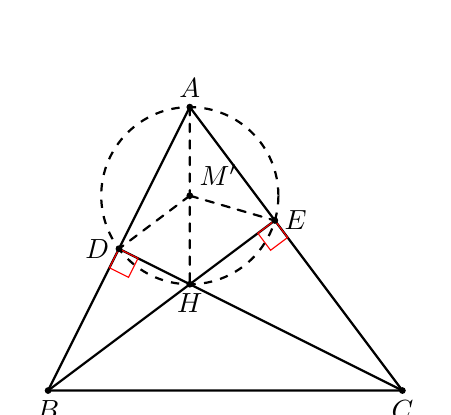
\begin{tikzpicture}[scale=0.9]
                        \tkzDefPoints{0/4/A, -2/0/B, 3/0/C}
                        \tkzDefPointBy[projection=onto A--B](C) \tkzGetPoint{D}
                        \tkzDefPointBy[projection=onto A--C](B) \tkzGetPoint{E}
                        \tkzDrawPolygon[black, thick](A,B,C)
                        \tkzDrawSegments[black, thick](C,D B,E)
                        \tkzMarkRightAngle[color=red, size=0.3](B,D,C)
                        \tkzMarkRightAngle[color=red, size=0.3](B,E,C)
                        \tkzInterLL(B,E)(C,D) \tkzGetPoint{H}
                        \tkzDefPointWith[linear, K=1/2](A,H) \tkzGetPoint{M'}
                        \tkzDrawPoints[fill=black](A,B,C,D,E,H,M')
                        \tkzLabelPoints[above](A)
                        \tkzLabelPoints[below](B,C,H)
                        \tkzLabelPoints[left](D)
                        \tkzLabelPoints[right](E)
                        \tkzLabelPoints[above right](M')
                        \tkzDrawCircle[black, thick, dashed](M',A)
                        \tkzDrawSegments[black, thick, dashed](A,H M',D M',E)
                    \end{tikzpicture}
                    \label{fig:Angle_s2.2-5}
                    \caption{例題2.2-1(ii)方法一示意圖}
                \end{subfigure}              
            \end{figure}
            作$AH$的中點$M'$。由$CD\perp AB$和$BE\perp AC$可知 $\triangle{HDA}$和$\triangle{HEA}$都是直角三角形，
            且$\angle{HDA}$和$\angle{HEA}$都是直角。

            由「直角三角形斜邊上的中線等於斜邊的一半」可知$M'H=M'D=M'E=M'A$，所以$A$、$D$、$E$、$H$四點共圓。
            \item 圓周角
            
            因為$CD\perp AB$、$BE\perp AC$，所以有$\angle{HDA}=\angle{HEA}=90^{\circ}$，即有
            $$
                \angle{HDA}=180^{\circ}-\angle{HEA}
            $$
        
            因為$D$、$E$在$AH$的異側，所以$A$、$D$、$E$、$H$四點共圓。
        \end{enumerate}
    \end{enumerate}
\end{mybox}
\begin{mybox}[例題\thesubsection-2]{6em}{1em}{0.5em}
    在$\triangle{ABC}$中，$D$和$E$分別是線段$AB$和$AC$上的點，滿足$\triangle{AED}\sim\triangle{ABC}$。

    求證：$B$、$C$、$D$、$E$四點共圓。
\end{mybox}
\begin{mybox}[解]{3em}{1em}{0.5em}
    \begin{figure}[H]
        \begin{subfigure}[b]{\textwidth}
            \centering
            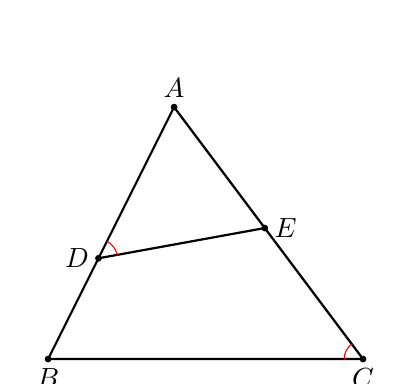
\begin{tikzpicture}[scale=0.8]
                \tkzDefPoints{0/4/A, -2/0/B, 3/0/C}
                \tkzDefPointWith[linear, K=3/5](A,B) \tkzGetPoint{D}
                \tkzDefTriangleCenter[circum](B,C,D) \tkzGetPoint{O}
                \tkzInterLC(A,C)(O,B) \tkzGetPoints{C_tmp}{E}
                \tkzDrawPolygon[black, thick](A,B,C)
                \tkzDrawSegments[black, thick](D,E)
                \tkzMarkAngle[color=red, size=0.3](E,D,A)
                \tkzMarkAngle[color=red, size=0.3](A,C,B)
                \tkzDrawPoints[fill=black](A,B,C,D,E)
                \tkzLabelPoints[above](A)
                \tkzLabelPoints[below](B,C)
                \tkzLabelPoints[left](D)
                \tkzLabelPoints[right](E)
            \end{tikzpicture}
            \label{fig:Angle_s2.2-6}
            \caption{例題2.2-2示意圖}
        \end{subfigure}              
    \end{figure}
    因為$\triangle{AED}\sim\triangle{ABC}$，所以$\angle{EDA}=\angle{ACB}=\angle{ECB}$。

    又因為$\angle{EDB}=180^{\circ}-\angle{EDA}$，所以有$\angle{EDB}+\angle{ECB}=180^{\circ}$。

    因此可知$B$、$C$、$D$、$E$四點共圓。
\end{mybox}
\begin{mybox}[例題\thesubsection-3]{6em}{1em}{1em}
    對於銳角$\triangle{ABC}$，記$H$為$\triangle{ABC}$的垂心，$H_A$、$H_B$、$H_C$分別為$H$關於$BC$、$CA$、$AB$的對稱點。
    求證：$A$、$B$、$C$、$H_A$、$H_B$、$H_C$六點共圓。
\end{mybox}
\begin{mybox}[解]{3em}{1em}{0.5em}
    \begin{figure}[H]
        \begin{subfigure}[b]{\textwidth}
            \centering
            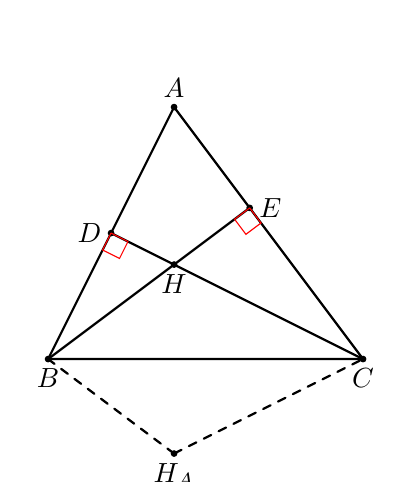
\begin{tikzpicture}[scale=0.8]
                \tkzDefPoints{0/4/A, -2/0/B, 3/0/C}
                \tkzDefPointBy[projection=onto A--B](C) \tkzGetPoint{D}
                \tkzDefPointBy[projection=onto A--C](B) \tkzGetPoint{E}
                \tkzInterLL(B,E)(C,D) \tkzGetPoint{H}
                \tkzDefPointBy[reflection=over B--C](H) \tkzGetPoint{H_A}
                \tkzDrawPoints[fill=black](A,B,C,D,E,H,H_A)
                \tkzDrawPolygon[black, thick](A,B,C)
                \tkzDrawSegments[black, thick](C,D B,E)
                \tkzDrawSegments[black, thick, dashed](H_A,B H_A,C)
                \tkzMarkRightAngle[color=red, size=0.3](B,D,C)
                \tkzMarkRightAngle[color=red, size=0.3](B,E,C)
                \tkzLabelPoints[above](A)
                \tkzLabelPoints[below](B,C,H,H_A)
                \tkzLabelPoints[left](D)
                \tkzLabelPoints[right](E)
            \end{tikzpicture}
            \label{fig:Angle_s2.2-7}
            \caption{例題2.2-3示意圖}
        \end{subfigure}              
    \end{figure}
    作$BH$、$CH$分別交$AC$、$AB$於$E$、$D$兩點。

    只需要對$\angle{BHC}$做Angle Chasing便可：
    \begin{align*}
        \angle{BHC}&=180^{\circ}-\angle{HCB}-\angle{CBH}\\
        &=180^{\circ}-\angle{DCB}-\angle{CBE}\\
        &=\left(90^{\circ}-\angle{DCB}\right)+\left(90^{\circ}-\angle{CBE}\right)\\
        &=\angle{CBD}+\angle{ECB}\\
        &=\angle{CBA}+\angle{ACB}\\
        &=180^{\circ}-\angle{BAC}
    \end{align*}
    因為$H_A$與$H$關於$BC$對稱，所以$\angle{BH_AC}=\angle{BHC}$，即有
    $$
        \angle{BH_AC}+\angle{BAC}=180^{\circ}
    $$
    因此，$A$、$B$、$C$、$H_A$四點共圓。

    同理可證得$A$、$B$、$C$、$H_C$和$A$、$B$、$C$、$H_C$分別都四點共圓，由此可知$A$、$B$、$C$、$H_A$、$H_B$、$H_C$六點共圓。
\end{mybox}
\subsection{圓冪}
\begin{mybox}[定理]{4em}{1em}{1em}
    對於不共線的四點$A$、$B$、$C$、$D$，設直線$AB$與直線$CD$交於點$P$，
    則$A$、$B$、$C$、$D$四點共圓的充分必要條件是
    $$
        \overrightarrow{PA}\cdot\overrightarrow{PB}=\overrightarrow{PC}\cdot\overrightarrow{PD}
    $$
    \begin{enumerate}[label = \arabic*., itemsep=0.3em]
        \item 相交弦定理；
        \item 兩割線定理。
    \end{enumerate}
    \begin{figure}[H]
        \centering
        \begin{subfigure}[b]{0.45\textwidth}
            \centering
            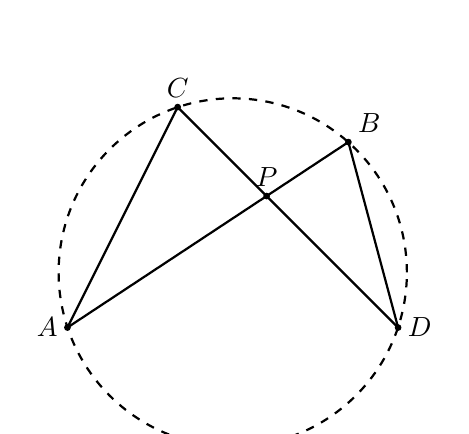
\begin{tikzpicture}[scale=0.7]
                \tkzDefPoint(0,4){C}
                \tkzDefPoint(-2,0){A}
                \tkzDefPoint(4,0){D}
                \tkzCircumCenter(C,A,D) \tkzGetPoint{O}
                \tkzDefPointBy[rotation=center O angle -60](C) \tkzGetPoint{B}
                \tkzDrawCircle[black, thick, dashed](O,B)
                \tkzInterLL(A,B)(C,D) \tkzGetPoint{P}
                \tkzDrawPoints[fill=black](A,B,C,D,P)
                \tkzDrawSegments[black, thick](A,B C,D A,C B,D)
                \tkzLabelPoints[left](A)
                \tkzLabelPoints[above](C,P)
                \tkzLabelPoints[right](D)
                \tkzLabelPoints[above right](B)
            \end{tikzpicture}
            \caption{相交弦定理}
            \label{fig:pow_s2.3-1}
        \end{subfigure}
        \stepcounter{figure}
        \hfill % 在兩圖之間加入彈性間距
        \begin{subfigure}[b]{0.45\textwidth}
            \centering
            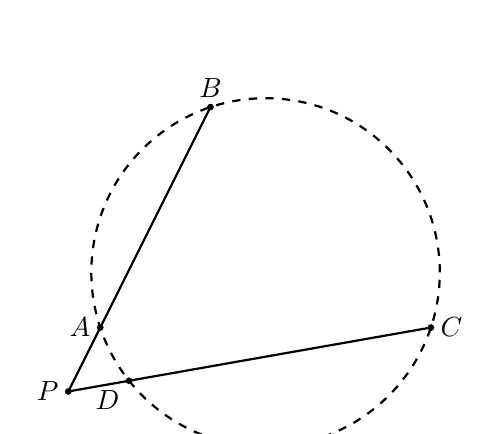
\begin{tikzpicture}[scale=0.7]
                \tkzDefPoint(0,4){B}
                \tkzDefPoint(-2,0){A}
                \tkzDefPoint(4,0){C}
                \tkzCircumCenter(A,B,C) \tkzGetPoint{O}
                \tkzDefPointBy[rotation=center O angle 20](A) \tkzGetPoint{D}
                \tkzDrawCircle[black, thick, dashed](O,B)
                \tkzInterLL(A,B)(C,D) \tkzGetPoint{P}
                \tkzDrawPoints[fill=black](A,B,C,D,P)
                \tkzDrawSegments[black, thick](P,B P,C)
                \tkzLabelPoints[left](A)
                \tkzLabelPoints[above](B)
                \tkzLabelPoints[right](C)
                \tkzLabelPoints[below left](D)
                \tkzLabelPoints[left](P)
            \end{tikzpicture}
            \caption{兩割線定理}
            \label{fig:pow_s2.3-2}
        \end{subfigure}
    \end{figure}
\end{mybox}
\begin{mybox}[證明]{4em}{1em}{0.5em}
    因為定理的必要性可由圓內接四邊形的性質得出，所以只需證明定理的充分性就可。
    
    設直線$PC$交$\triangle{ABC}$的外接圖於另一點$D'\neq C$，由圓冪定理可知
    $$
        \overrightarrow{PA}\cdot\overrightarrow{PB}=\overrightarrow{PC}\cdot\overrightarrow{PD'}
    $$
    結合已知條件$\overrightarrow{PA}\cdot\overrightarrow{PB}=\overrightarrow{PC}\cdot\overrightarrow{PD}$可知$D'=D$，
    即$A$、$B$、$C$、$D$四點共圓。
\end{mybox}
\begin{mybox}[例題\thesubsection-1]{6em}{1em}{1em}
    圓$\Omega$和圓$\Gamma$相交於點$A$和$B$。在直線$BA$的延長線上任取一點$K$，
    過$K$點作直線$l_1$交圓$\Omega$於點$C$和$D$，作直線$l_2\neq l_1$交圓$\Omega$於點$E$和$F$。
    
    求證：$C$、$D$、$E$、$F$四點共圓。
\end{mybox}
\begin{mybox}[解]{3em}{1em}{0.5em}
    \begin{figure}[H]
        \begin{subfigure}[b]{\textwidth}
            \centering
            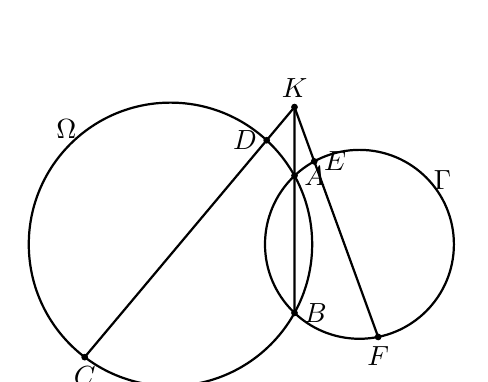
\begin{tikzpicture}[scale=0.3]
                \tkzDefPoints{-4/0/O_1, 2/0/A_tmp, 0/0/B_tmp, 4/0/O_2}
                \tkzInterCC(O_1,A_tmp)(O_2,B_tmp) \tkzGetPoints{A}{B}
                \tkzDefPointWith[linear, K=1.5](B,A) \tkzGetPoint{K}
                \tkzDefPointBy[rotation=center K angle -40](A) \tkzGetPoint{C_tmp}
                \tkzDefPointBy[rotation=center K angle +20](A) \tkzGetPoint{E_tmp}
                \tkzInterLC(K,C_tmp)(O_1,A) \tkzGetPoints{C}{D}
                \tkzInterLC(K,E_tmp)(O_2,A) \tkzGetPoints{E}{F}
                \tkzDefPointBy[rotation=center O_1 angle 90](D) \tkzGetPoint{O}
                \tkzDefPointBy[rotation=center O_2 angle -90](E) \tkzGetPoint{G}
                \tkzDrawPoints[fill=black](A,B,C,D,E,F,K)
                \tkzDrawCircle[black, thick](O_1,A)
                \tkzDrawCircle[black, thick](O_2,A)
                \tkzDrawSegments[black, thick](K,B K,C K,F)
                \tkzLabelPoints[above](K)
                \tkzLabelPoint[above](G){$\Gamma$}
                \tkzLabelPoint[above](O){$\Omega$}
                \tkzLabelPoints[below](C,F)
                \tkzLabelPoints[left](D)
                \tkzLabelPoints[right](A,B,E)
            \end{tikzpicture}
            \label{fig:pow_s2.3-3}
            \caption{例題2.3-1示意圖}
        \end{subfigure}              
    \end{figure}
    對圓$\Omega$使用圓冪定理可知
    $$
        \overrightarrow{KA}\cdot\overrightarrow{KB}=\overrightarrow{KC}\cdot\overrightarrow{KD}
    $$
    對圓$\Gamma$使用圓冪定理可知
    $$
        \overrightarrow{KA}\cdot\overrightarrow{KB}=\overrightarrow{KE}\cdot\overrightarrow{KF}
    $$
    所以
    $$
        \overrightarrow{KC}\cdot\overrightarrow{KD}=\overrightarrow{KE}\cdot\overrightarrow{KF}
    $$
    即$C$、$D$、$E$、$F$四點共圓。
\end{mybox}
\begin{mybox}[例題\thesubsection-2]{6em}{1em}{1em}
    同一個平面內有兩條不重合且不平行的直線$l_1$和$l_2$，
    點$A$、$B$、$C$是直線$l_1$上的三個相異點，點$D$、$E$和$F$是直線$l_2$上的三個相異點。
    已知$A$、$B$、$D$、$E$四點共圓，$AD\parallel CF$。求證：$B$、$C$、$E$、$F$四點共圓。
\end{mybox}
\begin{mybox}[解]{3em}{1em}{0.5em}
    設$l_1$與$l_2$相交於$K$點。

    因為$A$、$B$、$D$、$E$四點共圓，所以有
    $$
        \overrightarrow{KA}\cdot\overrightarrow{KB}=\overrightarrow{KD}\cdot\overrightarrow{KE}
    $$
    因為$AD\parallel CF$，所以$\triangle{KAD}$與$\triangle{KCF}$位似，位似中心為$K$，因此
    $$
        \frac{\overrightarrow{KC}}{\overrightarrow{KA}}=\frac{\overrightarrow{KF}}{\overrightarrow{KD}}
    $$
    此時有
    \begin{align*}
        &\frac{\overrightarrow{KC}}{\overrightarrow{KA}}\cdot\overrightarrow{KA}\cdot\overrightarrow{KB}
        =\frac{\overrightarrow{KF}}{\overrightarrow{KD}}\cdot\overrightarrow{KD}\cdot\overrightarrow{KE}\\
        \Leftrightarrow\quad&\overrightarrow{KC}\cdot\overrightarrow{KB}=\overrightarrow{KF}\cdot\overrightarrow{KE}
    \end{align*}
    即$B$、$C$、$E$、$F$四點共圓。
\end{mybox}
\newpage
\subsection{托勒密定理}
本節主要介紹托勒密定理的判定方法，首先引用更強的托勒密不等式。
\begin{mybox}[托勒密不等式]{8em}{1em}{1em}
    對於凸四邊形$ABCD$，都有
    $$AB \cdot CD + AD \cdot BC \geq AC \cdot BD$$
    等號成立當且僅當$A$、$B$、$C$、$D$四點共圓。
\end{mybox}
\begin{mybox}[證明]{4em}{1em}{1em}
    \begin{figure}[H]
        \centering
        \begin{subfigure}[b]{\textwidth}
            \centering
            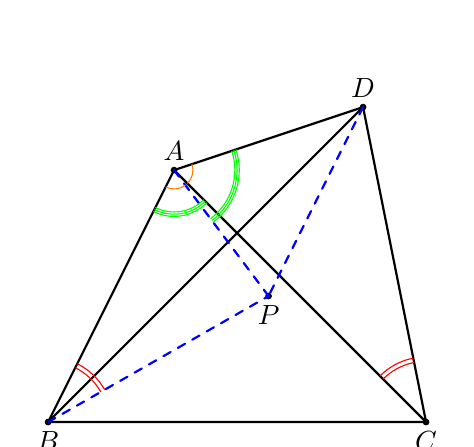
\begin{tikzpicture}[scale=0.8]
                \tkzDefPoint(0,4){A}
                \tkzDefPoint(-2,0){B}
                \tkzDefPoint(4,0){C}
                \tkzDefPoint(3,5){D}
                \tkzFindAngle(C,A,D) \tkzGetAngle{CAD}
                \tkzFindAngle(D,C,A) \tkzGetAngle{DCA}
                \tkzDefPointBy[rotation=center A angle \CAD](B) \tkzGetPoint{B_tmp}
                \tkzDefPointBy[rotation=center B angle -\DCA](A) \tkzGetPoint{A_tmp}
                \tkzInterLL(A,B_tmp)(B,A_tmp) \tkzGetPoint{P}
                \tkzDrawPolygon[black, thick](A,B,C,D)
                \tkzDrawPoints[fill=black](A,B,C,D,P)
                \tkzDrawSegments[black, thick](A,C B,D)
                \tkzDrawSegments[blue, thick, dashed](A,P B,P D,P)
                \tkzLabelPoints[above](A,D)
                \tkzLabelPoints[below](B,C,P)
                \tkzMarkAngle[size=0.3, color=orange, fill=orange!30](B,A,P)
                \tkzMarkAngle[size=0.3, color=orange, fill=orange!30](C,A,D)
                \tkzMarkAngle[color=red, arc=ll, fill=red!30](P,B,A)
                \tkzMarkAngle[color=red, arc=ll, fill=red!30](D,C,A)
                \tkzMarkAngle[size=0.7, color=green, arc=lll, fill=green!30](B,A,C)
                \tkzMarkAngle[color=green, arc=lll, fill=green!30](P,A,D)
            \end{tikzpicture}
            \caption{托勒密不等式示意圖}
            \label{fig:ptolemy_s2.4-1}
        \end{subfigure}
    \end{figure}
    作直線$l_1$，使$\measuredangle{\left(AB,l_1\right)}=\measuredangle{CAD}$；
    
    作直線$l_2$，使$\measuredangle{\left(BA,l_2\right)}=\measuredangle{ACD}$。

    設$l_1$與$l_2$交於點$P$，則有$\triangle{APB}\sim\triangle{ADC}$，所以
    \begin{equation}
        \frac{AP}{AD}=\frac{AB}{AC}=\frac{PB}{DC} \Rightarrow AB\cdot CD=AC\cdot BP\label{eq:ptolemy_ineq_1}
    \end{equation}
    同時亦能注意到$\triangle{ABC}\sim\triangle{APD}$，所以
    \begin{equation}
       \frac{AC}{AD}=\frac{BC}{PD} \Rightarrow AD\cdot BC=AP\cdot DP\label{eq:ptolemy_ineq_2}
    \end{equation}
    把\eqref{eq:ptolemy_ineq_1}和\eqref{eq:ptolemy_ineq_2}相加，得到
    \begin{equation}
        AB\cdot CD + AD\cdot BC = AC\cdot\left(BP + DP\right)\geq AC\cdot BD\label{eq:ptolemy_ineq_3}
    \end{equation}
    等號成立條件為$P$位於線段$BD$上，即等價於
    $$\measuredangle{ACD}=\measuredangle{ABP}=\measuredangle{ABD}\Leftrightarrow \text{$A$、$B$、$C$、$D$四點共圓}$$
\end{mybox}
\begin{mybox}[托勒密定理]{7em}{1em}{1em}
    對於凸四邊形$ABCD$，$A$、$B$、$C$、$D$四點共圓的充分必要條件是
    $$AB \cdot CD + AD \cdot BC = AC \cdot BD$$
\end{mybox}
\subsection{三弦定理}
\begin{mybox}[定理]{4em}{1em}{1em}
    對於凸四邊形$ABCD$，$A$、$B$、$C$、$D$四點共圓的充分必要條件是
    $$
        AB\sin{\angle{DAC}} + AD\sin{\angle{CAB}} = AC\sin{\angle{DAB}}
    $$
    \begin{figure}[H]
        \centering
        \begin{subfigure}[b]{\textwidth}
            \centering
            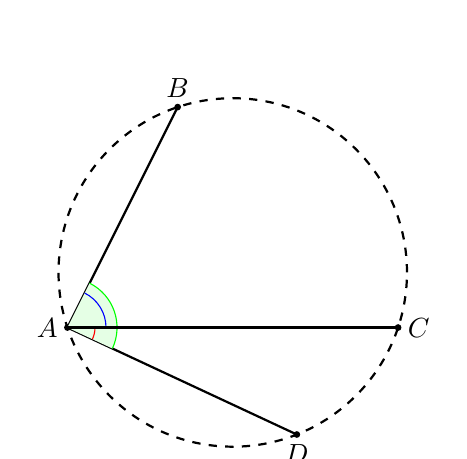
\begin{tikzpicture}[scale=0.7]
                \tkzDefPoint(0,4){B}
                \tkzDefPoint(-2,0){A}
                \tkzDefPoint(4,0){C}
                \tkzCircumCenter(A,B,C) \tkzGetPoint{O}
                \tkzDefPointBy[rotation=center O angle -50](C) \tkzGetPoint{D}
                \tkzDrawCircle[black, thick, dashed](O,B)
                \tkzDrawPoints[fill=black](A,B,C,D)
                \tkzDrawSegments[black, thick](A,B A,D)
                \tkzLabelPoints[left](A)
                \tkzLabelPoints[above](B)
                \tkzLabelPoints[right](C)
                \tkzLabelPoints[below](D)
                \tkzFillAngle[fill=green!10, size=0.9](D,A,B)
                \tkzMarkAngle[color=red, size=0.5](D,A,C)
                \tkzMarkAngle[color=blue, size=0.7](C,A,B)
                \tkzMarkAngle[color=green, size=0.9](D,A,B)
                \tkzDrawSegment[black, thick](A,C)
            \end{tikzpicture}
            \caption{三弦定理的示意圖}
            \label{fig:ttc_s2.5-1}
        \end{subfigure}
    \end{figure}
\end{mybox}
\begin{mybox}[證明]{4em}{1em}{1em}
    因為定理的必要性可結合托勒密定理和正弦定理直接推導得出，所以只需證明定理的充分性就可。

    設射線$AC$交$\triangle{ABD}$的外接圓於$C'\neq A$，由定理的必要性可知
    $$
        AC'\sin{\angle{DAB}}=AB\sin{\angle{DAC'}} + AD\sin{\angle{C'AB}}=AB\sin{\angle{DAC}} + AD\sin{\angle{CAB}}
    $$
    結合已知條件可知
    $$
        AC'\sin{\angle{DAB}}=AC\sin{\angle{DAB}}
    $$
    又因為$\angle{DAB}\neq 0^{\circ}$或$180^{\circ}$，所以$\sin{\angle{DAB}}\neq0$。因此有$AC'=AC$，即$C=C'$。
\end{mybox}
\begin{mybox}[思考]{4em}{1em}{1em}
    換成有向角（例：$\angle{DAC}\rightarrow\measuredangle{DAC}$）是否依然成立？
\end{mybox}
\begin{mybox}[回答]{4em}{1em}{1em}
    換成有向角（例：$\angle{DAC}\rightarrow\measuredangle{DAC}$）依然成立，此時甚至可以把前置條件「凸四邊形$ABCD$」刪去。
\end{mybox}
\begin{mybox}[例題\thesubsection-1]{6em}{1em}{1em}
    $\triangle{ABC}$的內心和$A$點所對旁心分別為$I$和$J_A$，$I$和$J_A$分在直線$AB$上的投影分別為$E$和$F$，$E$關於$A$的對稱點為$E'$。
    現在射線$AI$上存在一點$D\neq A$，其在$AB$上的投影為$D'$。如果$2AD'=E'F$，求證：$A$、$B$、$C$、$D$四點共圓。
\end{mybox}
\begin{mybox}[解答]{4em}{1em}{1em}
    \begin{figure}[H]
        \begin{subfigure}[b]{\textwidth}
            \centering  
            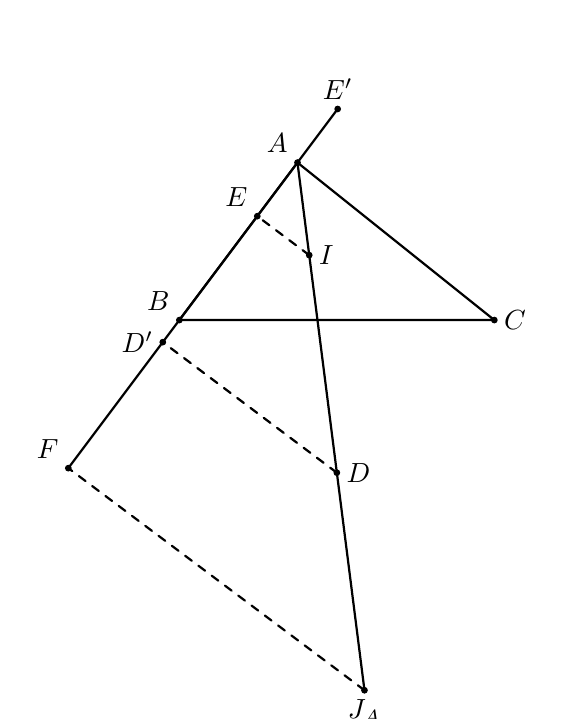
\begin{tikzpicture}[scale=0.5]
                \tkzDefPoints{0/4/A, -3/0/B, 5/0/C}
                \tkzDefTriangleCenter[circum](A,B,C) \tkzGetPoint{O}
                \tkzDefTriangleCenter[in](A,B,C) \tkzGetPoint{I}
                \tkzDefTriangleCenter[ex](B,A,C) \tkzGetPoint{J_A}
                \tkzDefPointWith[linear, K=1/2](I,J_A) \tkzGetPoint{D}
                \tkzDefPointBy[projection=onto A--B](D) \tkzGetPoint{D'}
                \tkzDefPointBy[projection=onto A--B](I) \tkzGetPoint{E}
                \tkzDefPointBy[projection=onto A--B](J_A) \tkzGetPoint{F}
                \tkzDefPointBy[symmetry=center A](E) \tkzGetPoint{E'}
                \tkzDrawPoints[fill=black](A,B,C,D,E,F,I,J_A,D',E')
                \tkzLabelPoints[above](E')
                \tkzLabelPoints[above left](A,E,F,B)
                \tkzLabelPoints[left](D')
                \tkzLabelPoints[right](I,D,C)
                \tkzLabelPoints[below](J_A)
                \tkzDrawPolygon[black, thick](A,B,C)
                \tkzDrawSegments[black, thick](E',A A,F A,J_A)
                \tkzDrawSegments[black, thick, dashed](I,E J_A,F D,D')
            \end{tikzpicture}
            \label{fig:ttc_s2.5-2}
            \caption{例題2.5-2示意圖}
        \end{subfigure}  
    \end{figure}
    本題可以用三弦定理或雞爪定理來解。
    \begin{enumerate}[label = 方法 \arabic*：]
        \item 三弦定理
        
        原命題等價於以下的命題一
        $$
            AB\sin{\angle{DAC}} + AC\sin{\angle{BAD}} = AD\sin{\angle{BAC}}
        $$
        因為$D$在$AI$上，利用內心的性質可知
        $$
            \angle{BAD}=\angle{DAC}=\frac{1}{2}\angle{BAC}
        $$
        代入至命題一，可等價轉換成以下的命題二
        $$
            AB+AC=2AD\cos{\frac{\angle{BAC}}{2}}=2AD'=E'F=E'A+AF=AE+AF
        $$
        命題二可由內心和外心的性質證得，容易證得原命題。
        \item 雞爪定理
        
        原命題等價於命題一——「$D$為$IJ_A$中點」。

        因為$IE$、$DD'$和$J_AF$同時垂直於$AB$，所以$IE\parallel DD'\parallel J_AF$。

        由平行線平線段成比例知
        $$
            \frac{ID}{DJ_A}=\frac{ED'}{D'F}
        $$
        因此命題一等價於命題二——「$ED'=D'F$」。

        由已知條件可知
        \begin{align*}
            &2AD'=E'F\\
            \Leftrightarrow\quad& 2AD'=E'A+AF=AE+AF=2AE+EF\\
            \Leftrightarrow\quad& 2ED'=2AD'-2AE=EF\\
            \Leftrightarrow\quad& ED'=EF-ED'=D'F
        \end{align*}
        命題二成立，原命題得證。
    \end{enumerate}
\end{mybox}
\section{與三點共線的聯繫}
\begin{mybox}[西姆松定理]{7em}{1em}{1em}
    同一平面上已知$\triangle{ABC}$以及$\triangle{ABC}$外一點$P$，$P$分別在直線$BC$、$CA$和$AB$上的投影分別為$D$、$E$和$F$。
    那麼，$A$、$B$、$C$、$P$四點共圓的充分必要條件是$D$、$E$、$F$三點共線。
    \begin{figure}[H]
        \centering
        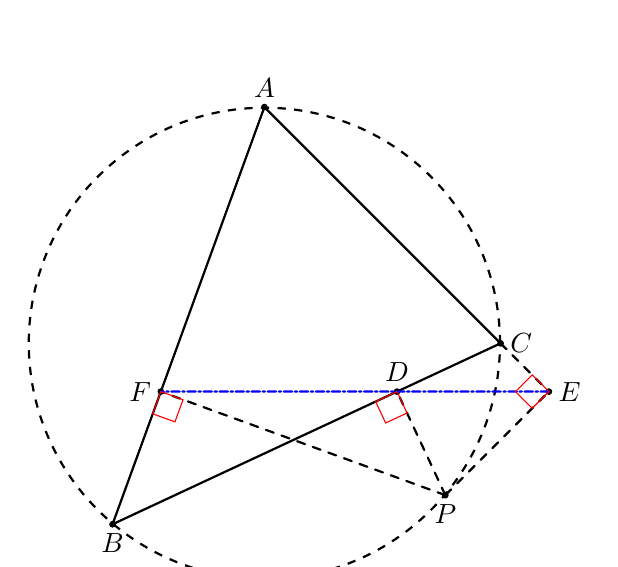
\begin{tikzpicture}[scale=1.0]
            \tkzDefPoints{0/0/O, 0/3/A}
            \tkzDefPointBy[rotation=center O angle 140](A) \tkzGetPoint{B}
            \tkzDefPointBy[rotation=center O angle -90](A) \tkzGetPoint{C}
            \tkzDefPointBy[rotation=center O angle -130](A) \tkzGetPoint{P}
            \tkzDefPointBy[projection=onto B--C](P) \tkzGetPoint{D}
            \tkzDefPointBy[projection=onto C--A](P) \tkzGetPoint{E}
            \tkzDefPointBy[projection=onto A--B](P) \tkzGetPoint{F}
            \tkzDrawCircle[black, thick, dashed](O,P)
            \tkzDrawPoints[fill=black](A,B,C,D,E,F,P)
            \tkzDrawPolygon[black, thick](A,B,C)
            \tkzDrawSegments[black, thick, dashed](P,D P,E P,F C,E)
            \tkzLabelPoints[above](A,D)
            \tkzLabelPoints[right](C,E)
            \tkzLabelPoints[below](B,P)
            \tkzLabelPoints[left](F)
            \tkzDrawSegment[blue, thick,densely dash dot](E,F)
            \tkzMarkRightAngle[color=red, size=0.3](B,F,P)
            \tkzMarkRightAngle[color=red, size=0.3](B,D,P)
            \tkzMarkRightAngle[color=red, size=0.3](A,E,P)      
        \end{tikzpicture}
        \label{fig:simpson_s3-1}
        \caption{西姆松定理示意圖}
    \end{figure}
\end{mybox}
\begin{mybox}[必要性證明]{7em}{1em}{1em}
    利用三角函數能簡單得到
    $$
        \begin{cases}
            \overrightarrow{BD}/\overrightarrow{DC}=\cot{\measuredangle{PBC}}/\cot{\measuredangle{BCP}}=-\cot{\measuredangle{PBC}}/\cot{\measuredangle{PCB}}\\
            \overrightarrow{CE}/\overrightarrow{EA}=\cot{\measuredangle{PCA}}/\cot{\measuredangle{CAP}}=-\cot{\measuredangle{PCA}}/\cot{\measuredangle{PAC}}\\
            \overrightarrow{AF}/\overrightarrow{FB}=\cot{\measuredangle{PAB}}/\cot{\measuredangle{ABP}}=-\cot{\measuredangle{PAB}}/\cot{\measuredangle{PBA}}
        \end{cases}
    $$
    以上三式相乘可得
    \begin{align*}
        \frac{\overrightarrow{BD}}{\overrightarrow{DC}}
        \cdot\frac{\overrightarrow{CE}}{\overrightarrow{EA}}
        \cdot\frac{\overrightarrow{AF}}{\overrightarrow{FB}}&=
        \left(-\frac{\cot{\measuredangle{PBC}}}{\cot{\measuredangle{PCB}}}\right)
        \cdot\left(-\frac{\cot{\measuredangle{PCA}}}{\cot{\measuredangle{PAC}}}\right)
        \cdot\left(-\frac{\cot{\measuredangle{PAB}}}{\cot{\measuredangle{PBA}}}\right)\\
        &=-\frac{\cot{\measuredangle{PBC}}}{\cot{\measuredangle{PAC}}}
        \cdot\frac{\cot{\measuredangle{PAB}}}{\cot{\measuredangle{PCB}}}
        \cdot\frac{\cot{\measuredangle{PCA}}}{\cot{\measuredangle{PBA}}}
    \end{align*}
    因為$A$、$B$、$C$、$P$四點共圓，所以有
    $$
        \begin{cases}
            \measuredangle{PBC}=\measuredangle{PAC}+180^{\circ}k_C,\ k_C\in\mathbb{Z}\\
            \measuredangle{PCA}=\measuredangle{PBA}+180^{\circ}k_A,\ k_A\in\mathbb{Z}\\
            \measuredangle{PAB}=\measuredangle{PCB}+180^{\circ}k_B,\ k_B\in\mathbb{Z}
        \end{cases}
    $$
    最後結合$\cot{}$函數的最小正周期為$180^{\circ}$可知
    $$
        \frac{\overrightarrow{BD}}{\overrightarrow{DC}}
        \cdot\frac{\overrightarrow{CE}}{\overrightarrow{EA}}
        \cdot\frac{\overrightarrow{AF}}{\overrightarrow{FB}} = -1
    $$
    由梅涅勞斯定理可知，$D$、$E$、$F$三點共圓。
\end{mybox}
\begin{mybox}[充分性證明]{7em}{1em}{1em}
    因為$PD\perp BC$及$PE\perp CA$，所以$P$、$D$、$E$、$C$四點共圓，因此
    $$
        \angle{PCB}=\angle{PCD}=\angle{PED}=\angle{PEF}
    $$
    因為$PE\perp CA$及$PF\perp AB$，所以$P$、$E$、$F$、$A$四點共圓，因此
    $$
        \angle{PEF}=\angle{PAF}=\angle{PAB}
    $$
    兩式結合可得
    $$
        \angle{PCB}=\angle{PAB}
    $$
    因此$A$、$B$、$C$、$P$四點共圓。
\end{mybox}
\section{與三線共點的聯繫}
\begin{mybox}[根軸]{4em}{1em}{1em}
    %\renewcommand{\thefigure}{\thesection-\arabic{figure}} % 主圖編號
    \renewcommand{\thesubfigure}{圖 \thesection-\arabic{figure}} % 子圖變為 2-1
    對於兩個非同心圓$\odot{O_1}$和$\odot{O_2}$，其半徑分別為$R_1$和$R_2$。由$\odot{O_1}$和$\odot{O_2}$誘導出來的「根軸」$l_{12}$是指
    $$
        l_{12}=\left\{P\text{是動點}\ |\ O_1P^2-R_1^2=O_2P^2-R_2^2\right\}
    $$
    \begin{figure}[H]
        \centering
        \begin{subfigure}[b]{0.45\textwidth}
            \centering
            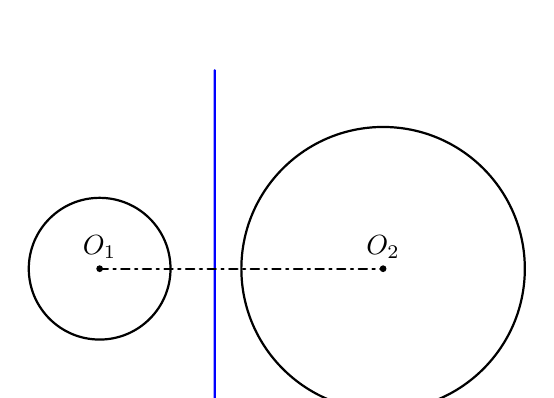
\begin{tikzpicture}[scale=0.9]
                \tkzDefPoints{-2/0/O_1, 2/0/O_2}
                \tkzDefPointWith[linear, K=13/32](O_1,O_2) \tkzGetPoint{P}
                \tkzDefLine[perpendicular=through P](O_1,O_2) \tkzGetPoint{Q}
                \tkzDrawLine[blue, thick, add=0.5 and -0.3](P,Q)
                %\tkzInterCC[R](O_1,1)(O_2,2) \tkzGetPoints{A}{B}
                \tkzDrawPoints[fill=black](O_1,O_2)
                \tkzDrawSegment[black, thick, dash dot](O_1, O_2)
                \tkzDrawArc[R,color=black, thick](O_1,1)(0,360)
                \tkzDrawArc[R,color=black, thick](O_2,2)(0,360)
                \tkzLabelPoints[above](O_1,O_2)
            \end{tikzpicture}
            \caption{兩圓相離}
            \label{fig:RA_s4-1}
        \end{subfigure}
        \stepcounter{figure}
        \hfill % 在兩圖之間加入彈性間距
        \begin{subfigure}[b]{0.45\textwidth}
            \centering
            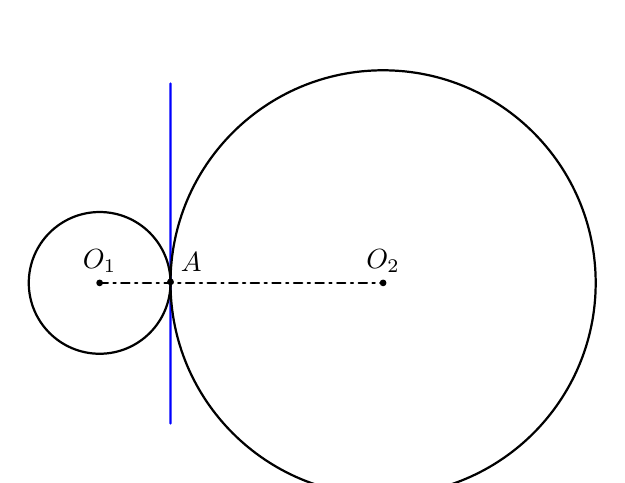
\begin{tikzpicture}[scale=0.9]
                \tkzDefPoints{-2/0/O_1, 2/0/O_2}
                \tkzInterCC[R](O_1,1)(O_2,3) \tkzGetPoints{A}{B}
                \tkzDefLine[perpendicular=through A](O_1,O_2) \tkzGetPoint{Q}
                \tkzDrawLine[blue, thick, add=0.5 and -0.3](A,Q)
                %\tkzInterCC[R](O_1,1)(O_2,2) \tkzGetPoints{A}{B}
                \tkzDrawPoints[fill=black](O_1,O_2,A)
                \tkzDrawSegment[black, thick, dash dot](O_1, O_2)
                \tkzDrawArc[R,color=black, thick](O_1,1)(0,360)
                \tkzDrawArc[R,color=black, thick](O_2,3)(0,360)
                \tkzLabelPoints[above](O_1,O_2)
                \tkzLabelPoints[above right](A)
            \end{tikzpicture}
            \caption{兩圓外切}
            \label{fig:RA_s4-2}
        \end{subfigure}
    \end{figure}

    \begin{figure}[H]
        \centering
        \begin{subfigure}[b]{0.45\textwidth}
            \centering
            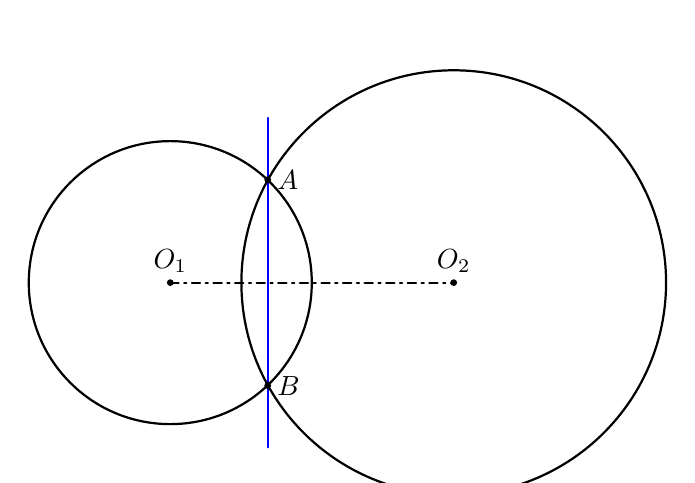
\begin{tikzpicture}[scale=0.9]
                \tkzDefPoints{-2/0/O_1, 2/0/O_2}
                \tkzInterCC[R](O_1,2)(O_2,3) \tkzGetPoints{A}{B}
                \tkzDrawLine[blue, thick, add=0.3 and 0.3](A,B)
                \tkzDrawSegment[black, thick, dash dot](O_1, O_2)
                \tkzDrawPoints[fill=black](O_1,A,B,O_2)
                \tkzLabelPoints[above](O_1,O_2)
                \tkzLabelPoints[right](A,B)
                \tkzDrawCircles[black, thick](O_1,A O_2,B)
            \end{tikzpicture}
            \caption{兩圓相交}
            \label{fig:RA_s4-3}
        \end{subfigure}
        \stepcounter{figure}
        \hfill % 在兩圖之間加入彈性間距
        \begin{subfigure}[b]{0.45\textwidth}
            \centering
            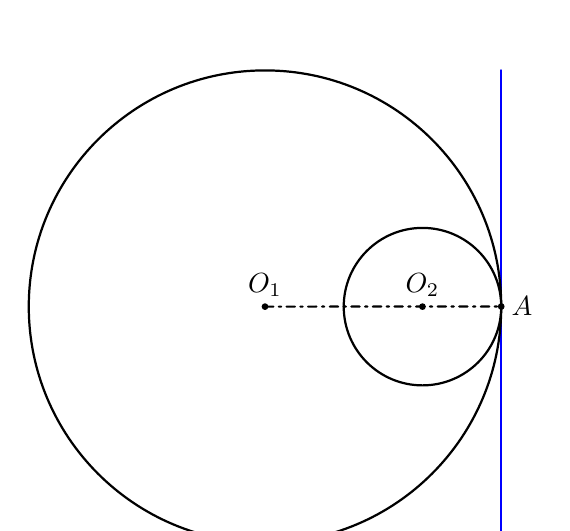
\begin{tikzpicture}[scale=0.5]
                \tkzDefPoints{-2/0/O_1, 2/0/O_2}
                \tkzInterCC[R](O_1,6)(O_2,2) \tkzGetPoints{A}{B}
                \tkzDefLine[perpendicular=through A](O_1,O_2) \tkzGetPoint{Q}
                \tkzDrawLine[blue, thick, add=1.5 and 0.5](A,Q)
                %\tkzInterCC[R](O_1,1)(O_2,2) \tkzGetPoints{A}{B}
                \tkzDrawPoints[fill=black](O_1,O_2,A)
                \tkzDrawSegment[black, thick, dash dot](O_1, A)
                \tkzDrawArc[R,color=black, thick](O_1,6)(0,360)
                \tkzDrawArc[R,color=black, thick](O_2,2)(0,360)
                \tkzLabelPoints[above](O_1,O_2)
                \tkzLabelPoints[right](A)
            \end{tikzpicture}
            \caption{兩圓內切}
            \label{fig:RA_s4-4}
        \end{subfigure}
    \end{figure}
\end{mybox}
\begin{mybox}[定理1]{4em}{1em}{1em}
    根軸$l_{12}$是一條垂直於連心線$O_1O_2$的直線。
\end{mybox}
\begin{mybox}[證明]{4em}{1em}{1em}
    在$l_{12}$上任取一點$P$，由根軸的定義可知
    \begin{align*}
        &O_1P^2-R_1^2=O_2P^2-R_2^2\\
        \Leftrightarrow\quad&O_1P^2-O_2P^2=R_1^2-R_2^2\\
        \Leftrightarrow\quad&\overrightarrow{O_1P}^2-\overrightarrow{O_2P}^2=R_1^2-R_2^2\\
        \Leftrightarrow\quad&\left(\overrightarrow{O_1P}-\overrightarrow{O_2P}\right)\cdot\left(\overrightarrow{O_1P}+\overrightarrow{O_2P}\right)=R_1^2-R_2^2\\
        \Leftrightarrow\quad&\overrightarrow{O_1O_2}\cdot\left(\overrightarrow{O_1P}+\overrightarrow{O_2P}\right)=R_1^2-R_2^2\\
        \Leftrightarrow\quad&\overrightarrow{O_1O_2}\cdot\left(\overrightarrow{PO_1}+\overrightarrow{PO_2}\right)=R_2^2-R_1^2
    \end{align*}
    記$O_1O_2$的中點為$M$，由中點的向量表達式可知
    $$
        2\overrightarrow{PE}=\overrightarrow{PO_1}+\overrightarrow{PO_2}
    $$
    所以有
    $$
        2\overrightarrow{O_1O_2}\cdot\overrightarrow{PE}=R_2^2-R_1^2
    $$
    在$O_1O_2$上取一點$P'$，滿足
    $$
        \overrightarrow{P'E}=\frac{R_2^2-R_1^2}{2\left|\overrightarrow{O_1O_2}\right|^2}\overrightarrow{O_1O_2}
    $$
    此時有
    $$
        2\overrightarrow{O_1O_2}\cdot\overrightarrow{P'E}
        =2\overrightarrow{O_1O_2}\cdot\left(\frac{R_2^2-R_1^2}{2\left|\overrightarrow{O_1O_2}\right|^2}\overrightarrow{O_1O_2}\right)
        =R_2^2-R_1^2
    $$
    即$P'$在$l_{12}$上，而且
    \begin{align*}
        &2\overrightarrow{O_1O_2}\cdot\overrightarrow{PE}=R_2^2-R_1^2=2\overrightarrow{O_1O_2}\cdot\overrightarrow{P'E}\\
        \Leftrightarrow\quad&2\overrightarrow{O_1O_2}\cdot\left(\overrightarrow{PE}-\overrightarrow{P'E}\right)=0\\
        \Leftrightarrow\quad&\overrightarrow{O_1O_2}\cdot\overrightarrow{PP'}=0
    \end{align*}
    由向量內積的性質可知，$PP'\perp O_1O_2$。

    根軸上所有點$P$都在過$P'$點且垂直於連心線$O_1O_2$的直線上，所以根軸$l_{12}$就是直線$PP'$，即$l_{12}\perp O_1O_2$。
\end{mybox}
\begin{mybox}[定理2]{4em}{1em}{1em}
    兩圓外切，根軸為內公切線；兩圓相交，根軸為兩個交點連成的直線；兩圓內切，根軸為外公切線。
\end{mybox}
\begin{mybox}[證明]{4em}{1em}{1em}
    對於兩圓的交點$A$（無論是外切、相交或是內切），顯然有
    $$
        O_1A^2-R_1^2=0=O_2A^2-R_2^2
    $$
    所以$A$點必然是根軸$l_{12}$上的一點。由定理一可知，$l_{12}$為過$A$點且垂直於連心線$O_1O_2$的直線。

    當兩圓外切時，滿足條件的直線就是內公切線；

    當兩圓相交時，滿足條件的直線就是公共弦所在直線；

    當兩圓內切時，滿足條件的直線就是外公切線。
\end{mybox}
\begin{mybox}[定理3]{4em}{1em}{1em}
    對於三個圓心不共線的圓$\odot{O_1}$、$\odot{O_2}$和$\odot{O_3}$，根軸$l_{12}$、$l_{23}$、$l_{31}$三線共點。交點稱為「根心」。
\end{mybox}
\begin{mybox}[證明]{4em}{1em}{1em}
    因為$O_1$、$O_2$、$O_3$不共線，結合定理一可知，$l_{12}$、$l_{23}$、$l_{31}$兩兩不平行且不重合。

    設$K$為$l_{12}$和$l_{23}$的交點，那麼由根軸的定義可知
    $$
        O_1K^2-R_1=O_2K^2-R_2^2=O_3K^2-R_3^2
    $$
    由$l_{31}$的定義可知$K$在根軸$l_{31}$上，所以根軸$l_{12}$、$l_{23}$、$l_{31}$三線共點。
\end{mybox}
\begin{mybox}[例題\thesection-1]{6em}{1em}{1em}
    已知$BCDE$是圓內接四邊形，$A$是$BCDE$外接圓外的一點。
    若$BC$交$DE$於$P$，$AP$交$\triangle{ADE}$的外接圓於$K\neq A$點，則$A$、$B$、$C$、$K$四點共圓。

    此定理稱為「根心定理」。
\end{mybox}
\begin{mybox}[證明]{4em}{1em}{1em}
    本題可由根心定理或圓冪定理來解。
    \begin{enumerate}[label = 方法 \arabic*：]
        \item 根心定理
        
        第一，圓$BCDE$和圓$ABC$的公共弦是$BC$。由定理2可知，圓$BCDE$和圓$ABC$所誘導的根軸是直線$BC$；

        第二，圓$BCDE$和圓$ADE$的公共弦是$DE$。由定理2可知，圓$BCDE$和圓$ADE$所誘導的根軸是直線$DE$；

        第三，設圓$ADE$和圓$ABC$的公共弦是$AK'$。由定理2可知，圓$ADE$和圓$ABC$所誘導的根軸是直線$AK'$；

        由根心定理知，$BC$、$DE$、$AK'$三線共點。結合已知條件，三線交點為$P$，所以$P$、$A$、$K'$三點共線。

        因為$K'$在$\triangle{ADE}$的外接圓上，同時亦在直線$AP$上，所以有$K'=K$。

        因為$K'$、$A$、$B$、$C$四點共圓，所以$A$、$B$、$C$、$K$四點共圓。
        \item 圓冪定理
        
        對$\triangle{ADE}$的外接圓使用圓冪定理
        $$
            \overrightarrow{PA}\cdot\overrightarrow{PK}=\overrightarrow{PD}\cdot\overrightarrow{PE}
        $$
        對四邊形$BCDE$的外接圓使用圓冪定理
        $$
            \overrightarrow{PB}\cdot\overrightarrow{PC}=\overrightarrow{PD}\cdot\overrightarrow{PE}
        $$
        所以有
        $$
            \overrightarrow{PA}\cdot\overrightarrow{PK}=\overrightarrow{PB}\cdot\overrightarrow{PC}
        $$
        因此$A$、$B$、$C$、$K$四點共圓。
    \end{enumerate}
\end{mybox}
\section{練習題}
\begin{mybox}[Problem 1]{7em}{1em}{1em}
   對於$\triangle{ABC}$，記$I$為$\triangle{ABC}$的內心，$J_A$為$\angle{CBA}$和$\angle{BCA}$的外角平分線的交點。

   求證：$B$、$I$、$J_A$、$C$四點共圓。
\end{mybox}
\begin{mybox}[Answer 1]{7em}{1em}{1em}
    \begin{figure}[H]
        \centering
        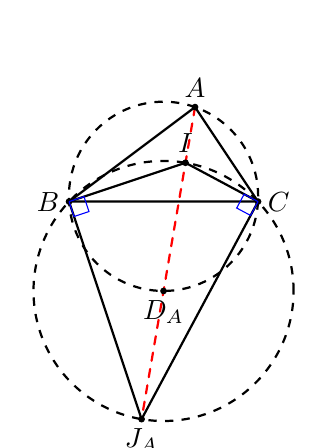
\begin{tikzpicture}[scale=0.4]
            \tkzDefPoints{0/3/A, -4/0/B, 2/0/C}
            \tkzDefTriangleCenter[in](A,B,C) \tkzGetPoint{I}
            \tkzDefTriangleCenter[circum](A,B,C) \tkzGetPoint{O}
            \tkzDefTriangleCenter[circum](I,B,C) \tkzGetPoint{D_A}
            \tkzDefTriangleCenter[ex](B,A,C) \tkzGetPoint{J_A}
            \tkzDrawCircle[black, thick, dashed](O,A)
            \tkzDrawCircle[black, thick, dashed](D_A,I)
            \tkzDrawSegment[red, thick, dashed](A,J_A)
            \tkzDrawPoints[fill=black](A,B,C,I,J_A,D_A)
            \tkzDrawPolygon[black, thick](A,B,C)
            \tkzDrawSegments[black, thick](B,I C,I B,J_A C,J_A)
            \tkzLabelPoints[above](A,I)
            \tkzLabelPoints[left](B)
            \tkzLabelPoints[right](C)
            \tkzLabelPoints[below](J_A,D_A)
            \tkzMarkRightAngle[color=blue, size=0.5](J_A,B,I)
            \tkzMarkRightAngle[color=blue, size=0.5](I,C,J_A)
        \end{tikzpicture}
        \label{fig:p1,2-1}
        \caption{Problem 1和Problem 2示意圖}
    \end{figure}
    由內心的性質可知，$BI$和$CI$分別是$\angle{CBA}$和$\angle{ACB}$的內角平分線，所以有$BI\perp BJ_A$和$CI\perp CJ_A$，即$\angle{J_ABI}=\angle{ICJ_A}=90^{\circ}$。
    
    利用圓周角的判定定理可知，$B$、$I$、$J_A$、$C$四點共圓。
\end{mybox}
\begin{mybox}[Problem 2]{7em}{1em}{1em}
   承上題，記$IJ_A$的中點$D_A$。
   
   求證：$A$、$B$、$C$、$D_A$四點共圓且$A$、$I$、$D_A$、$J_A$四點共線。
\end{mybox}
\begin{mybox}[Answer 2]{7em}{1em}{1em}
    因為$B$、$I$、$C$、$J_A$四點共圓，且$\angle{J_ABI}=90^{\circ}$，所以$IJ_A$是圓$BICJ_A$的直徑，因此$D_A$是圓$BICJ_A$的圓心。
    
    由圓周角定理可知
    \begin{align*}
        \angle{CD_AB}&=2\angle{CJ_AB}\\
        &=2\times\left(180^{\circ}-\angle{BIC}\right)\\
        &=2\times\left(\angle{CBI}+\angle{ICB}\right)\\
        &=2\times\left(\frac{\angle{CBA}}{2}+\frac{\angle{ACB}}{2}\right)\\
        &=\angle{CBA}+\angle{ACB}\\
        &=180^{\circ}-\angle{BAC}
    \end{align*}
    
    利用圓周角的判定定理可知，$A$、$B$、$C$、$D_A$四點共圓。

    另一方面，利用旁心的判定定理可知，$J_A$在$\angle{BAC}$的內角平分線上，即$A$、$I$、$J_A$三點共線。
    
    又因為$D_A$是$IJ_A$的中點，所以$A$、$I$、$D_A$、$J_A$四點共線。
\end{mybox}
\begin{mybox}[Problem 3]{7em}{1em}{1em}
    對於鈍角$\triangle{ABC}$，記$H$為$\triangle{ABC}$的垂心，$H_A$、$H_B$、$H_C$分別為$H$關於$BC$、$CA$、$AB$的對稱點。
    求證：$A$、$B$、$C$、$H_A$、$H_B$、$H_C$六點共圓。
\end{mybox}
\begin{mybox}[Answer 3]{7em}{1em}{1em}
    本題可以使用無向角、有向角去解。
    \begin{enumerate}[label=方法 \arabic*：]
        \item 無向角
        
        \begin{figure}[H]
        \centering
        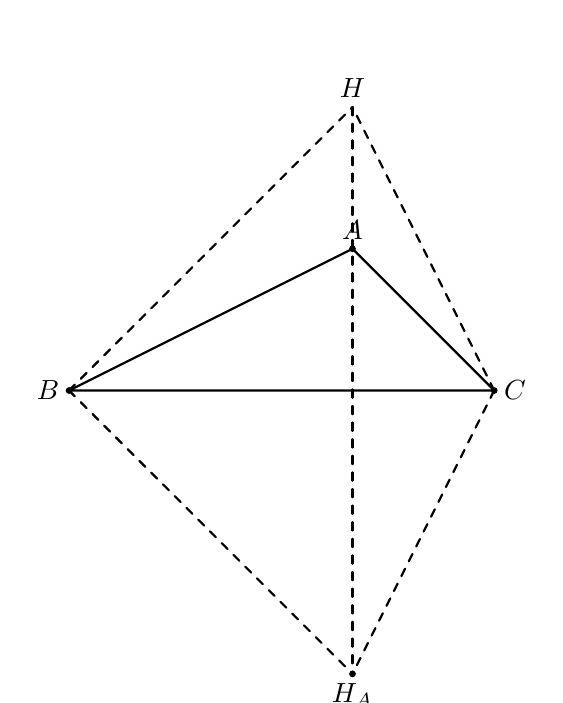
\begin{tikzpicture}[scale=0.6]
            \tkzDefPoints{0/3/A, -6/0/B, 3/0/C}
            \tkzDefTriangleCenter[ortho](A,B,C) \tkzGetPoint{H}
            \tkzDefPointBy[reflection=over B--C](H) \tkzGetPoint{H_A}
            \tkzDefPointBy[reflection=over C--A](H) \tkzGetPoint{H_B}
            \tkzDefPointBy[reflection=over A--B](H) \tkzGetPoint{H_C}  
            \tkzDrawPoints[fill=black](A,B,C,H_A)
            \tkzDrawPolygon[black, thick](A,B,C)
            \tkzDrawSegments[black, thick, dashed](B,H C,H B,H_A C,H_A H,H_A)
            \tkzLabelPoints[above](A,H)
            \tkzLabelPoints[left](B)
            \tkzLabelPoints[right](C)
            \tkzLabelPoints[below](H_A)
        \end{tikzpicture}
        \label{fig:p3-1}
        \caption{Problem 3中只含$H$和$H_A$示意圖}
        \end{figure}
        因為$H$是垂心，所以$BH\perp CA$和$CH\perp AB$，即
        $$
            \angle{CBH}=90^{\circ}-\angle{ACB},\ \angle{HCB}=90^{\circ}-\angle{CBA}
        $$
        結合$H_A$和$H$關於$BC$對稱可得
        \begin{align*}
            \angle{CH_AB}&=\angle{BHC}\\
            &=180^{\circ}-\angle{CBH}-\angle{HCB}\\
            &=180^{\circ}-\left(90^{\circ}-\angle{ACB}\right)-\left(90^{\circ}-\angle{CBA}\right)\\
            &=\angle{ACB}+\angle{CBA}\\
            &=180^{\circ}-\angle{BAC}
        \end{align*}
        由圓周角的判定定理可知，$A$、$B$、$C$、$H_A$。
        \begin{figure}[H]
            \centering
            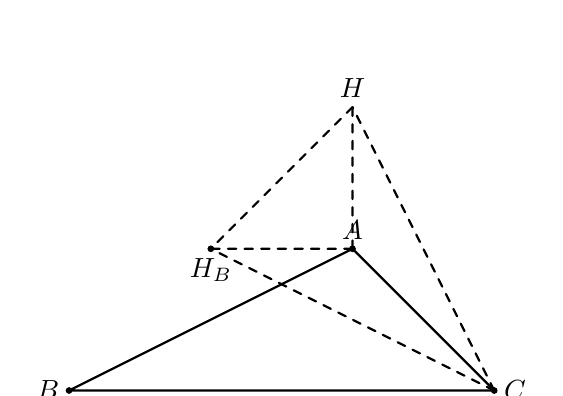
\begin{tikzpicture}[scale=0.6]
                \tkzDefPoints{0/3/A, -6/0/B, 3/0/C}
                \tkzDefTriangleCenter[ortho](A,B,C) \tkzGetPoint{H}
                \tkzDefPointBy[reflection=over B--C](H) \tkzGetPoint{H_A}
                \tkzDefPointBy[reflection=over C--A](H) \tkzGetPoint{H_B}
                \tkzDefPointBy[reflection=over A--B](H) \tkzGetPoint{H_C}  
                \tkzDrawPoints[fill=black](A,B,C,H_B)
                \tkzDrawPolygon[black, thick](A,B,C)
                \tkzDrawSegments[black, thick, dashed](C,H A,H C,H_B A,H_B H,H_B)
                \tkzLabelPoints[above](A,H)
                \tkzLabelPoints[left](B)
                \tkzLabelPoints[right](C)
                \tkzLabelPoints[below](H_B)
            \end{tikzpicture}
            \label{fig:p3-2}
            \caption{Problem 3中只含$H$和$H_B$示意圖}
        \end{figure}
        因為$H$是垂心，所以$CH\perp AB$和$AH\perp BC$，即
        $$
            \angle{HCA}=\angle{BAC}-90^{\circ},\ \angle{CAH}=\angle{ACB}+90^{\circ}
        $$
        結合$H_B$和$H$關於$CA$對稱可得
        \begin{align*}
            \angle{CH_BA}&=\angle{AHC}\\
            &=180^{\circ}-\angle{HCA}-\angle{CAH}\\
            &=180^{\circ}-\left(\angle{BAC}-90^{\circ}\right)-\left(\angle{ACB}+90^{\circ}\right)\\
            &=180^{\circ}-\angle{BAC}-\angle{ACB}\\
            &=\angle{CBA}
        \end{align*}
        由圓周角的判定定理可知，$A$、$B$、$C$、$H_B$。
        \begin{figure}[H]
            \centering
            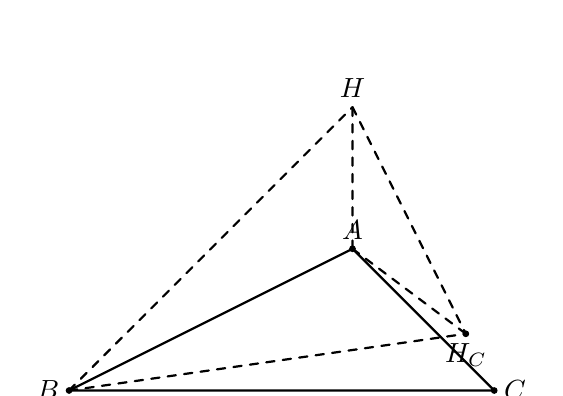
\begin{tikzpicture}[scale=0.6]
                \tkzDefPoints{0/3/A, -6/0/B, 3/0/C}
                \tkzDefTriangleCenter[ortho](A,B,C) \tkzGetPoint{H}
                \tkzDefPointBy[reflection=over B--C](H) \tkzGetPoint{H_A}
                \tkzDefPointBy[reflection=over C--A](H) \tkzGetPoint{H_B}
                \tkzDefPointBy[reflection=over A--B](H) \tkzGetPoint{H_C}  
                \tkzDrawPoints[fill=black](A,B,C,H_C)
                \tkzDrawPolygon[black, thick](A,B,C)
                \tkzDrawSegments[black, thick, dashed](A,H B,H A,H_C B,H_C H,H_C)
                \tkzLabelPoints[above](A,H)
                \tkzLabelPoints[left](B)
                \tkzLabelPoints[right](C)
                \tkzLabelPoints[below](H_C)
            \end{tikzpicture}
            \label{fig:p3-3}
            \caption{Problem 3中只含$H$和$H_C$示意圖}
        \end{figure}
        因為$H$是垂心，所以$AH\perp BC$和$BH\perp CA$，即
        $$
            \angle{HAB}=\angle{CBA}+90^{\circ},\ \angle{ABH}=\angle{BAC}-90^{\circ}
        $$
        結合$H_C$和$H$關於$AB$對稱可得
        \begin{align*}
            \angle{AH_CB}&=\angle{BHA}\\
            &=180^{\circ}-\angle{HAB}-\angle{ABH}\\
            &=180^{\circ}-\left(\angle{CBA}+90^{\circ}\right)-\left(\angle{BAC}-90^{\circ}\right)\\
            &=180^{\circ}-\angle{CBA}-\angle{BAC}\\
            &=\angle{ACB}
        \end{align*}

        \item 有向角
        
        只需證明$A$、$B$、$C$、$H_A$四點共圓即可。利用垂心的性質可得$BH\perp CA$和$CH\perp AB$，所以有
        $$
            \measuredangle{HCB}=90^{\circ}-\measuredangle{CBA},\ \measuredangle{CBH}=90^{\circ}-\measuredangle{ACB}
        $$
        在$\triangle{ABC}$中有
        $$
            \measuredangle{BAC}+\measuredangle{ACB}+\measuredangle{CBA}=0^{\circ}
        $$
        所以
        \begin{align*}
            \measuredangle{BHC}&=180^{\circ}-\measuredangle{HCB}-\measuredangle{CBH}\\
            &=180^{\circ}-\left(90^{\circ}-\measuredangle{CBA}\right)-\left(90^{\circ}-\measuredangle{ACB}\right)\\
            &=\measuredangle{CBA}+\measuredangle{ACB}\\
            &=-\measuredangle{BAC}=\measuredangle{CAB}
        \end{align*}
        因為$H_A$和$H$關於$BC$對稱，所以
        $$
            \measuredangle{CH_AB}=\measuredangle{BHC}=\measuredangle{CAB}
        $$
        由圓周角的判定定理可知$A$、$B$、$C$、$H_A$四點共圓。

        如此類推可得$A$、$B$、$C$、$H_A$、$H_B$、$H_C$六點共圓。
    \end{enumerate}
 
\end{mybox}
\begin{mybox}[Analysis 3]{7em}{1em}{1em}
    如果用無向角，解法相對較為直觀，但需要考慮圓周角的分佈及位置，必然需要配合幾何圖才可解釋；

    如果用有向角，解法相對較為kick手（因為大家對有向角的認識不太深），但是無需要考慮圓周角的位置。
\end{mybox}
\begin{mybox}[Problem 4*]{7em}{1em}{1em}
    令$H$是銳角$\triangle{ABC}$的垂心，$F$是$C$在$AB$邊上的投影，$P$是$H$關於$BC$的對稱點。
    假設$\triangle{AFP}$的外接圓交直線$BC$於$X$和$Y$兩個相異點，求證：$C$是線段$XY$的中點。
\end{mybox}
\begin{mybox}[Answer 4*]{7em}{1em}{1em}
    因為$P$是$H$關於$BC$的對稱點，所以$HP\perp BC$。

    因為$H$是銳角$\triangle{ABC}$的垂心，所以$AH\perp BC$。

    因此，$A$、$H$、$P$三點共線。記$AP$交$BC$於$E$，利用垂直關係和投影關係可知
    $$
        \measuredangle{CFA}=90^{\circ}=\measuredangle{CEA}
    $$
    所以$A$、$F$、$E$、$C$四點共圓，由圓冪定理可知
    $$
        \overrightarrow{BA}\cdot\overrightarrow{BF}=\overrightarrow{BE}\cdot\overrightarrow{BC}
    $$
    由題意可知$A$、$F$、$P$、$X$、$Y$五點共圓，由圓冪定理可知
    $$
        \overrightarrow{BA}\cdot\overrightarrow{BF}=\overrightarrow{BX}\cdot\overrightarrow{BY}
    $$
    與上式結合可得
    $$
        \overrightarrow{BE}\cdot\overrightarrow{BC}=\overrightarrow{BX}\cdot\overrightarrow{BY}
    $$
    由例題2.2-3或Problem 3可知，$A$、$B$、$C$、$P$四點共圓，由圓冪定理可知
    $$
        \overrightarrow{EA}\cdot\overrightarrow{EP}=\overrightarrow{EB}\cdot\overrightarrow{EC}
    $$
    再由$A$、$F$、$P$、$X$、$Y$五點共圓及圓冪定理可知
    $$
        \overrightarrow{EA}\cdot\overrightarrow{EP}=\overrightarrow{EX}\cdot\overrightarrow{EY}
    $$
    由上式結合可得
    $$
        \overrightarrow{EB}\cdot\overrightarrow{EC}=\overrightarrow{EX}\cdot\overrightarrow{EY}
    $$
    整理現有式子
    $$
        \begin{cases}
            \overrightarrow{EB}\cdot\overrightarrow{EC}=\overrightarrow{EX}\cdot\overrightarrow{EY}\\
            \overrightarrow{BE}\cdot\overrightarrow{BC}=\overrightarrow{BX}\cdot\overrightarrow{BY}
        \end{cases}
    $$
    記$XY$的中點為$C^\ast$，上方的等式組可以改寫成
    $$
        \begin{cases}
            \overrightarrow{EB}\cdot\overrightarrow{EC}=\overrightarrow{EX}\cdot\overrightarrow{EY}
            =\left(\frac{\overrightarrow{EX}+\overrightarrow{EY}}{2}\right)^2-\left(\frac{\overrightarrow{EX}-\overrightarrow{EY}}{2}\right)^2
            =\overrightarrow{EC^\ast}^2-\frac{1}{4}\overrightarrow{YX}^2\\
            \overrightarrow{BE}\cdot\overrightarrow{BC}=\overrightarrow{BX}\cdot\overrightarrow{BY}
            =\left(\frac{\overrightarrow{BX}+\overrightarrow{BY}}{2}\right)^2-\left(\frac{\overrightarrow{BX}-\overrightarrow{BY}}{2}\right)^2
            =\overrightarrow{BC^\ast}^2-\frac{1}{4}\overrightarrow{YX}^2
        \end{cases}
    $$
    等式組的下式減去上式可得
    \begin{align*}
        &\overrightarrow{BC^\ast}^2-\overrightarrow{EC^\ast}^2=\overrightarrow{BE}\cdot\left(\overrightarrow{BC}+\overrightarrow{EC}\right)\\
        \Leftrightarrow\quad&\left(\overrightarrow{BC^\ast}-\overrightarrow{EC^\ast}\right)\cdot\left(\overrightarrow{BC^\ast}+\overrightarrow{EC^\ast}\right)
        =\overrightarrow{BE}\cdot\left(\overrightarrow{BC}+\overrightarrow{EC}\right)\\
        \Leftrightarrow\quad&\overrightarrow{BE}\cdot\left(\overrightarrow{BC^\ast}+\overrightarrow{EC^\ast}\right)
        =\overrightarrow{BE}\cdot\left(\overrightarrow{BC}+\overrightarrow{EC}\right)\\
        \Leftrightarrow\quad&\overrightarrow{BC^\ast}+\overrightarrow{EC^\ast}=\overrightarrow{BC}+\overrightarrow{EC}\\
        \Leftrightarrow\quad&\overrightarrow{BC^\ast}-\overrightarrow{BC}+\overrightarrow{EC^\ast}-\overrightarrow{EC}=\overrightarrow{0}\\
        \Leftrightarrow\quad&2\overrightarrow{CC^\ast}=\overrightarrow{0}
    \end{align*}
    由此可算得$\overrightarrow{CC^\ast}=\overrightarrow{0}$，所以有$C=C^\ast$，即$C$是線段$XY$的中點。
\end{mybox}
\begin{mybox}[Problem 5*]{7em}{1em}{1em}
    如下圖，在四邊形$ABCD$中，$AB=AD$，$CB=CD$，$\angle{ABC}=90^\circ$。點$E$和$F$分別在線段$AB$和$AD$上，點$P$和$Q$在線段$EF$上（$P$在$E$和$Q$之間），\
    滿足$AE:EP=AF:FQ$。點$X$和$Y$分別在線段$CP$和$CQ$上，滿足$BX\perp CP$及$BY\perp CQ$。
    
    求證：$X$、$Y$、$P$、$Q$四點共圓。
    \begin{figure}[H]
        \centering
        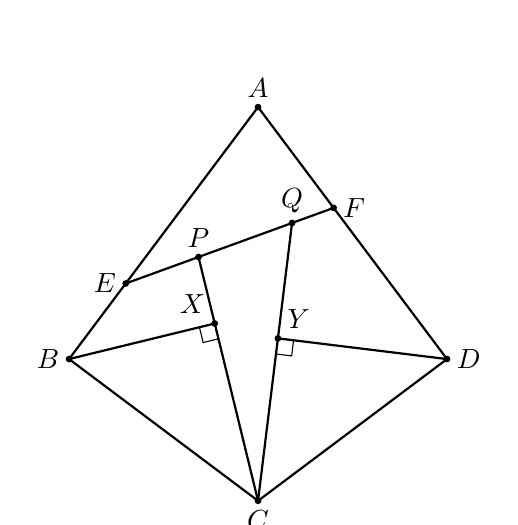
\begin{tikzpicture}[scale=1]
            \tkzDefPoints{0/0/A, -2.4/-3.2/B, 0/-5/C, 2.4/-3.2/D}
            \coordinate (E) at ($(A)!0.7!(B)$);
            \coordinate (F) at ($(A)!0.4!(D)$);
            \coordinate (P) at ($(E)!0.35!(F)$);
            \coordinate (Q) at ($(F)!0.2!(E)$);
            \tkzDefPointBy[projection=onto C--P](B) \tkzGetPoint{X}
            \tkzDefPointBy[projection=onto C--Q](D) \tkzGetPoint{Y}
            \tkzDrawPoints[fill=black](A,B,C,D,E,F,P,Q,X,Y)
            \tkzDrawPolygon[black, thick](A,B,C,D)
            \tkzDrawSegments[black, thick](E,F C,P C,Q B,X D,Y)
            \tkzLabelPoints[above](A,P,Q)
            \tkzLabelPoints[left](B,E)
            \tkzLabelPoints[right](D,F)
            \tkzLabelPoints[below](C)
            \tkzLabelPoints[above left](X)
            \tkzLabelPoints[above right](Y)
            \tkzMarkRightAngle[size=0.2](B,X,C)
            \tkzMarkRightAngle[size=0.2](C,Y,D)
        \end{tikzpicture}
        \label{fig:p5-1}
        \caption{Problem 5*示意圖}
    \end{figure}
\end{mybox}
\begin{mybox}[Answer 5*]{7em}{1em}{1em}
    原命題等價於以下的命題一
    $$
        CP\cdot CX=CQ\cdot CY
    $$
    因為$CX=CB\cos{\angle{PCB}}$、$CY=CD\cos{\angle{QCD}}$，結合$CB=CD$可知，命題一等價於以下的命題二
    $$
        CP\cos{\angle{PCB}}=CQ\cos{\angle{QCD}}
    $$
    \begin{figure}[H]
        \centering
        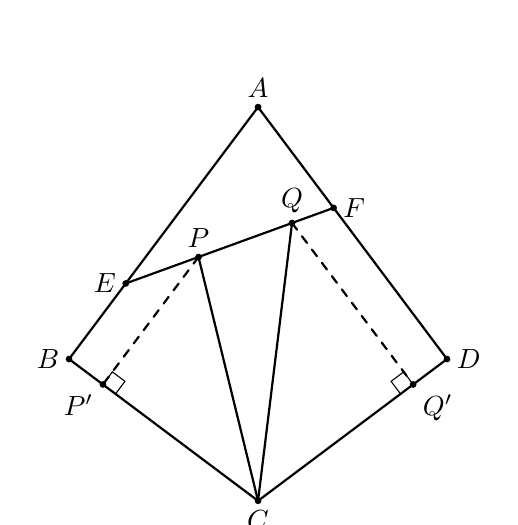
\begin{tikzpicture}[scale=1]
            \tkzDefPoints{0/0/A, -2.4/-3.2/B, 0/-5/C, 2.4/-3.2/D}
            \coordinate (E) at ($(A)!0.7!(B)$);
            \coordinate (F) at ($(A)!0.4!(D)$);
            \coordinate (P) at ($(E)!0.35!(F)$);
            \coordinate (Q) at ($(F)!0.2!(E)$);
            %\tkzDefPointBy[projection=onto C--P](B) \tkzGetPoint{X}
            %\tkzDefPointBy[projection=onto C--Q](D) \tkzGetPoint{Y}
            \tkzDefPointBy[projection=onto C--B](P) \tkzGetPoint{P'}
            \tkzDefPointBy[projection=onto C--D](Q) \tkzGetPoint{Q'}
            \tkzDrawPoints[fill=black](A,B,C,D,E,F,P,Q,P',Q')
            \tkzDrawPolygon[black, thick](A,B,C,D)
            \tkzDrawSegments[black, thick](E,F C,P C,Q)
            \tkzDrawSegments[black, thick, dashed](P,P' Q,Q')
            \tkzLabelPoints[above](A,P,Q)
            \tkzLabelPoints[left](B,E)
            \tkzLabelPoints[right](D,F)
            \tkzLabelPoints[below](C)
            %\tkzLabelPoints[above left](X)
            %\tkzLabelPoints[above right](Y)
            \tkzLabelPoints[below left](P')
            \tkzLabelPoints[below right](Q')
            \tkzMarkRightAngle[size=0.2](C,P',P)
            \tkzMarkRightAngle[size=0.2](Q,Q',C)
        \end{tikzpicture}
        \label{fig:p5-2}
        \caption{Problem 5*示意圖（去除$X$、$Y$兩點，增加$P'$、$Q'$）}
    \end{figure}
    作$P$、$Q$分別在$CB$、$CD$上的投影為$P'$、$Q'$，命題二等價於以下的命題三
    $$
        CP'=CQ'
    $$
    再次結合$CB=CD$可知，命題三等價於以下的命題四
    $$
        BP'=DQ'
    $$
    容易得知
    $$
        \begin{cases}
            BP'=PE\sin{\angle{PEA}}=PE\sin{\angle{FEA}}\\
            DQ'=QF\sin{\angle{QFA}}=QF\sin{\angle{EFA}}
        \end{cases}
    $$
    所以有
    $$
        \frac{BP'}{DQ'}=\frac{EP}{FQ}\cdot\frac{\sin{\angle{FEA}}}{\sin{\angle{EFA}}}
    $$
    對$\triangle{AEF}$使用正弦定理可得
    $$
        \frac{BP'}{DQ'}=\frac{EP}{FQ}\cdot\frac{\sin{\angle{FEA}}}{\sin{\angle{EFA}}}=\frac{EP}{FQ}\cdot\frac{AF}{AE}=\frac{AF/FQ}{AE/EP}=1
    $$
    由此可以命題四成立，即原命題得證。
\end{mybox}
\begin{mybox}[Problem 6]{7em}{1em}{1em}
    $AP$是$\triangle{ABC}$中的邊$BC$上的陪位中線，$D$、$E$分別在直線$AB$、$AC$上，$AP$平分線段$DE$，

    求證：$B$、$C$、$D$、$E$四點共圓。
\end{mybox}
\begin{mybox}[Answer 6]{7em}{1em}{1em}
    \begin{figure}[H]
        \centering
        \begin{tikzpicture}[scale=1]
            \tkzDefPoints{0/4/A, -3/0/B, 2/0/C}
            \tkzDefPointWith[linear, K=2/3](A,B) \tkzGetPoint{D}
            \tkzDefTriangleCenter[circum](B,C,D) \tkzGetPoint{O}
            \tkzInterLC[common=C](A,C)(O,C) \tkzGetFirstPoint{E}
            \tkzDefPointWith[linear, K=1/2](D,E) \tkzGetPoint{M}
            \tkzInterLL(A,M')(B,C) \tkzGetPoint{P}
            \tkzDrawPoints[fill=black](A,B,C,D,E,P,M)
            \tkzDrawPolygon[black, thick](A,B,C)
            \tkzDrawSegments[black, thick](D,E A,P)
            \tkzLabelPoints[above](A)
            \tkzLabelPoints[left](D)
            \tkzLabelPoints[right](E)
            \tkzLabelPoints[below](B,C,P,M)
            %\tkzLabelPoints[above left](X)
            %\tkzLabelPoints[above right](Y)
        \end{tikzpicture}
        \label{fig:p6-1}
        \caption{Problem 6示意圖}
    \end{figure}
    設$AP$交$DE$於$M$。

    因為$AP$是$BC$邊上的陪位中線，所以滿足
    $$
        \frac{\sin{\measuredangle{BAP}}}{\sin{\measuredangle{PAC}}}=\frac{AB}{AC}
    $$
    因為$AM$是$DE$邊上的中線，所以滿足
    $$
        \frac{\sin{\measuredangle{DAM}}}{\sin{\measuredangle{MAE}}}=\frac{AE}{AD}
    $$
    結合$\measuredangle{BAP}=\measuredangle{DAM}$和$\measuredangle{PAC}=\measuredangle{MAE}$可得
    $$
        AB\cdot AD=AC\cdot AE
    $$
    由圓冪的判定定理可知，$B$、$C$、$D$、$E$四點共圓。
\end{mybox}
\begin{mybox}[Problem 7]{7em}{1em}{1em}
    直線$l_1$上依次排列着$B_1$、$C_1$、$D_1$三點，直線$l_2$上依次排列着$B_2$、$C_2$、$D_2$三點。
    若$B_1B_2C_2C_1$和$C_1C_2D_2D_1$都是圓內接四邊形，

    求證：$B_1B_2\parallel D_1D_2$。
\end{mybox}
\begin{mybox}[Answer 7]{7em}{1em}{1em}
    在圓內接四邊形$B_1B_2C_2C_1$內有
    $$
        \measuredangle{B_1B_2C_2}=\measuredangle{B_1C_1C_2}
    $$
    因為直線$l_1$上依次排列着$B_1$、$C_1$、$D_1$三點，所以有
    $$
        \measuredangle{B_1C_1C_2}=-\measuredangle{C_2C_1D_1}
    $$
    在圓內接四邊形$C_1C_2D_2D_1$內有
    $$
        \measuredangle{C_2C_1D_1}=\measuredangle{C_2D_2D_1}
    $$
    結合以上三式有
    \begin{align*}
        &\measuredangle{B_1B_2C_2}=\measuredangle{C_2D_2D_1}\\
        \Leftrightarrow\quad& \measuredangle{\left(B_1B_2,l_2\right)}=-\measuredangle{\left(l_2,D_1D_2\right)}=\measuredangle{\left(D_1D_2,l_2\right)}
    \end{align*}
    由此可知 $B_1B_2\parallel D_1D_2$。
\end{mybox}
\begin{mybox}[Analysis 7]{7em}{1em}{1em}
    這題再次體現使用有向角的好處，能減少畫圖時的多點分佈情況。
\end{mybox}
\end{document}